%%%%%%%%%%%%%%%%%%%%%%%%%%%%%%%%%%%%%%%%%%%%%%%%%%%%%%%%%%%%%%%%%%%%%%%%%%%%%
%%% LaTeX-Rahmen fuer das Erstellen von englischen Bachelorarbeiten
%%%%%%%%%%%%%%%%%%%%%%%%%%%%%%%%%%%%%%%%%%%%%%%%%%%%%%%%%%%%%%%%%%%%%%%%%%%%%

%%%%%%%%%%%%%%%%%%%%%%%%%%%%%%%%%%%%%%%%%%%%%%%%%%%%%%%%%%%%%%%%%%%%%%%%%%%%%
%%% allgemeine Einstellungen
%%%%%%%%%%%%%%%%%%%%%%%%%%%%%%%%%%%%%%%%%%%%%%%%%%%%%%%%%%%%%%%%%%%%%%%%%%%%%

\documentclass[twoside,12pt,a4paper]{report}
%\usepackage{reportpage}
\usepackage[english]{babel}
\usepackage{epsf}
\usepackage{graphics, graphicx}
\usepackage{latexsym}
\usepackage[margin=10pt,font=small,labelfont=bf]{caption}
\usepackage[utf8]{inputenc}
\usepackage{amsmath}
\usepackage{amsfonts}
\usepackage{amssymb}
\usepackage{amstext}
\usepackage[numbers]{natbib}
\usepackage{titling}
\usepackage{hyperref}
\usepackage{caption}
\usepackage{subcaption}
\usepackage{multirow}

\textwidth 14cm
\textheight 22cm
\topmargin 0.0cm
\evensidemargin 1cm
\oddsidemargin 1cm
%\footskip 2cm
\parskip0.5explus0.1exminus0.1ex

% Kann von Student auch nach pers\"onlichem Geschmack ver\"andert werden.
\pagestyle{headings}

\sloppy

\begin{document}

%%%%%%%%%%%%%%%%%%%%%%%%%%%%%%%%%%%%%%%%%%%%%%%%%%%%%%%%%%%%%%%%%%%%%%%%%%%%
%%% Layout Title page
%%%%%%%%%%%%%%%%%%%%%%%%%%%%%%%%%%%%%%%%%%%%%%%%%%%%%%%%%%%%%%%%%%%%%%%%%%%%
 
\begin{titlepage}
 \begin{center}
  {\LARGE Eberhard Karls Universit\"at T\"ubingen}\\
  {\large Mathematisch-Naturwissenschaftliche Fakultät \\
Wilhelm-Schickard-Institut f\"ur Informatik\\[4cm]}
  {\huge Bachelor Thesis Bioinformatics\\[2cm]}
  {\Large\bf  Semi-supervised learning for nucleic acid cross-linking mass spectrometry\\[1.5cm]}
 {\large Emil Paulitz}\\[0.5cm]
14.08.2020\\[3cm]
\begin{center}
{\small\bf Reviewer}\\[0.5cm]
 {\large Prof. Oliver Kohlbacher}\\
  {\footnotesize Department of Computer Science\\
	University of T\"ubingen}
  \end{center}
	
\begin{center}
{\small\bf Supervisor}\\[0.5cm]
  {\large Timo Sachsenberg}\\
  {\footnotesize Address\\
	University of T\"ubingen}\end{center}

  \end{center}
\end{titlepage}
%%%%%%%%%%%%%%%%%%%%%%%%%%%%%%%%%%%%%%%%%%%%%%%%%%%%%%%%%%%%%%%%%%%%%%%%%%%%
%%% Layout back of title page
%%%%%%%%%%%%%%%%%%%%%%%%%%%%%%%%%%%%%%%%%%%%%%%%%%%%%%%%%%%%%%%%%%%%%%%%%%%%

\thispagestyle{empty}
\vspace*{\fill}
\begin{minipage}{11.2cm}
\textbf{Paulitz, Emilian Nicolaus Simons:}\\
\emph{Semi-supervised learning for nucleic acid cross-linking mass spectrometry}\\ Bachelor Thesis Bioinformatics\\
Eberhard Karls Universit\"at T\"ubingen\\
Period: 14.04.2020-14.08.2020
\end{minipage}
\newpage

%%%%%%%%%%%%%%%%%%%%%%%%%%%%%%%%%%%%%%%%%%%%%%%%%%%%%%%%%%%%%%%%%%%%%%%%%%%%

\pagenumbering{roman}
\setcounter{page}{1}

%%%%%%%%%%%%%%%%%%%%%%%%%%%%%%%%%%%%%%%%%%%%%%%%%%%%%%%%%%%%%%%%%%%%%%%%%%%%
%%% Page I: Abstract
%%%%%%%%%%%%%%%%%%%%%%%%%%%%%%%%%%%%%%%%%%%%%%%%%%%%%%%%%%%%%%%%%%%%%%%%%%%%


\section*{Abstract}

Write here your abstract.
\newpage
%%%%%%%%%%%%%%%%%%%%%%%%%%%%%%%%%%%%%%%%%%%%%%%%%%%%%%%%%%%%%%%%%%%%%%%%%%%%
%%% Page 2: Danksagung
%%%%%%%%%%%%%%%%%%%%%%%%%%%%%%%%%%%%%%%%%%%%%%%%%%%%%%%%%%%%%%%%%%%%%%%%%%%%
\section*{Acknowledgements}

Write here your acknowledgements.

\cleardoublepage

%%%%%%%%%%%%%%%%%%%%%%%%%%%%%%%%%%%%%%%%%%%%%%%%%%%%%%%%%%%%%%%%%%%%%%%%%%%%%
%%% Table of Contents
%%%%%%%%%%%%%%%%%%%%%%%%%%%%%%%%%%%%%%%%%%%%%%%%%%%%%%%%%%%%%%%%%%%%%%%%%%%%%

\renewcommand{\baselinestretch}{1.3}
\small\normalsize

\tableofcontents

\renewcommand{\baselinestretch}{1}
\small\normalsize

\cleardoublepage

%%%%%%%%%%%%%%%%%%%%%%%%%%%%%%%%%%%%%%%%%%%%%%%%%%%%%%%%%%%%%%%%%%%%%%%%%%%%%
%%% List of Figures
%%%%%%%%%%%%%%%%%%%%%%%%%%%%%%%%%%%%%%%%%%%%%%%%%%%%%%%%%%%%%%%%%%%%%%%%%%%%%

\renewcommand{\baselinestretch}{1.3}
\small\normalsize

\addcontentsline{toc}{chapter}{List of Figures}
\listoffigures

\renewcommand{\baselinestretch}{1}
\small\normalsize

\cleardoublepage

%%%%%%%%%%%%%%%%%%%%%%%%%%%%%%%%%%%%%%%%%%%%%%%%%%%%%%%%%%%%%%%%%%%%%%%%%%%%%
%%% List of tables
%%%%%%%%%%%%%%%%%%%%%%%%%%%%%%%%%%%%%%%%%%%%%%%%%%%%%%%%%%%%%%%%%%%%%%%%%%%%%

\renewcommand{\baselinestretch}{1.3}
\small\normalsize

\addcontentsline{toc}{chapter}{List of Tables}
\listoftables

\renewcommand{\baselinestretch}{1}
\small\normalsize

\cleardoublepage

%%%%%%%%%%%%%%%%%%%%%%%%%%%%%%%%%%%%%%%%%%%%%%%%%%%%%%%%%%%%%%%%%%%%%%%%%%%%%
%%% List of abbreviations
%%%%%%%%%%%%%%%%%%%%%%%%%%%%%%%%%%%%%%%%%%%%%%%%%%%%%%%%%%%%%%%%%%%%%%%%%%%%%

\addcontentsline{toc}{chapter}{List of Abbreviations}
\chapter*{List of Abbreviations\markboth{LIST OF ABBREVIATIONS}{LIST OF ABBREVIATIONS}}

\begin{tabbing}
\textbf{FACTOTUM}\hspace{1cm}\=Schrott\kill
\textbf{MS}\> Mass Spectrometry \\
\textbf{LC} \> Liquid Chromatography\\
\textbf{MS/MS} \> Tandem Mass Spectrometry\\
\textbf{PSM} \> Peptide Spectrum Match\\
\textbf{FDR} \> False Discovery Rate\\
\textbf{ROC} \> Receiver Operating Characteristics\\
\textbf{TPR} \> True Positive Rate\\
\textbf{FPR} \> False Positive Rate\\
\textbf{SVM} \> Support Vector Machine\\
\textbf{AUC} \> Area Under the Curve\\
\end{tabbing}

\cleardoublepage

%%%%%%%%%%%%%%%%%%%%%%%%%%%%%%%%%%%%%%%%%%%%%%%%%%%%%%%%%%%%%%%%%%%%%%%%%%%%%
%%% Der Haupttext, ab hier mit arabischer Numerierung
%%% Mit \input{dateiname} werden die Dateien `dateiname' eingebunden
%%%%%%%%%%%%%%%%%%%%%%%%%%%%%%%%%%%%%%%%%%%%%%%%%%%%%%%%%%%%%%%%%%%%%%%%%%%%%

\pagenumbering{arabic}
\setcounter{page}{1}

%% Introduction and Background
%%%%%%%%%%%%%%%%%%%%%%%%%%%%%%%%%%%%%%%%%%%%%%%%%%%%%%%%%%%%%%%%%%%%
% Einleitung
%%%%%%%%%%%%%%%%%%%%%%%%%%%%%%%%%%%%%%%%%%%%%%%%%%%%%%%%%%%%%%%%%%%%

\chapter{Introduction}
\label{introduction}
- Motivation
%Am Ende der Einleitung folgt ein Text so \"ahnlich wie (Nat\"urlich das folgende alles auf Englisch !!):
%
%Die Arbeit gliedert sich dazu wie folgt: Die Grundlagen von ...
%werden in Kapitel~\ref{introduction} erarbeitet. 
%...
%Eine
%Diskussion und ein kurzer Ausblick im
%Kapitel~\ref{discussion} beschlie{\ss}en diese Arbeit.
%
%Bevor wir uns der Auswertung bzw. Bewertung der gewonnenen Prim\"ardaten zuwenden, wollen wir zun\"achst einige grundlegende Begriffe der deskriptiven Statistik wiederholen.

\section{Background}
\label{background}

	Proteomics is an interdisciplinary research field analyzing the composition, interaction and impacts of the proteome (the entirety of proteins) of single cells or up to a whole organism~\cite{Han2008, Sachsenberg2017}. In this thesis, research was done in a related field, focusing on peptides cross-linked with RNA. The chemical bond between cross-linked molecules has been artificially induced, for example using UV light~\cite{Sachsenberg2017}. Applying this to peptides and RNA could possibly give insight into their \textit{in vivo} interactions, and may also allow conclusions about protein-DNA interaction.\\
	For quantitatively characterizing the proteome of a sample, large scale measuring techniques are needed. Mostly, mass spectrometry (MS) is used, or more specifically, as for the data in this thesis, tandem mass spectrometry (MS/MS) combined with liquid chromatography (LC). In order to analyze the protein sample with MS, its complexity has to be reduced as much as possible, for example using LC~\cite{Sachsenberg2017}. As~\citet{Han2008} explains, the mass spectrometer then produces mass spectra, which have to be analyzed further. It does so by first ionizing the substrate, because it can only detect charged particles. Then, the sample is separated in the mass analyzer by the ratio $\frac{m}{z}$, mass of the particles to their charge. The detector then quantifies the amount of a particle in the sample. The result is a mass spectrum, as shown in figure~\ref{fig:mass_spectrum}.\\
	{
	\renewcommand{\baselinestretch}{0.9} 
	\normalsize
	\begin{figure}
		\centering
		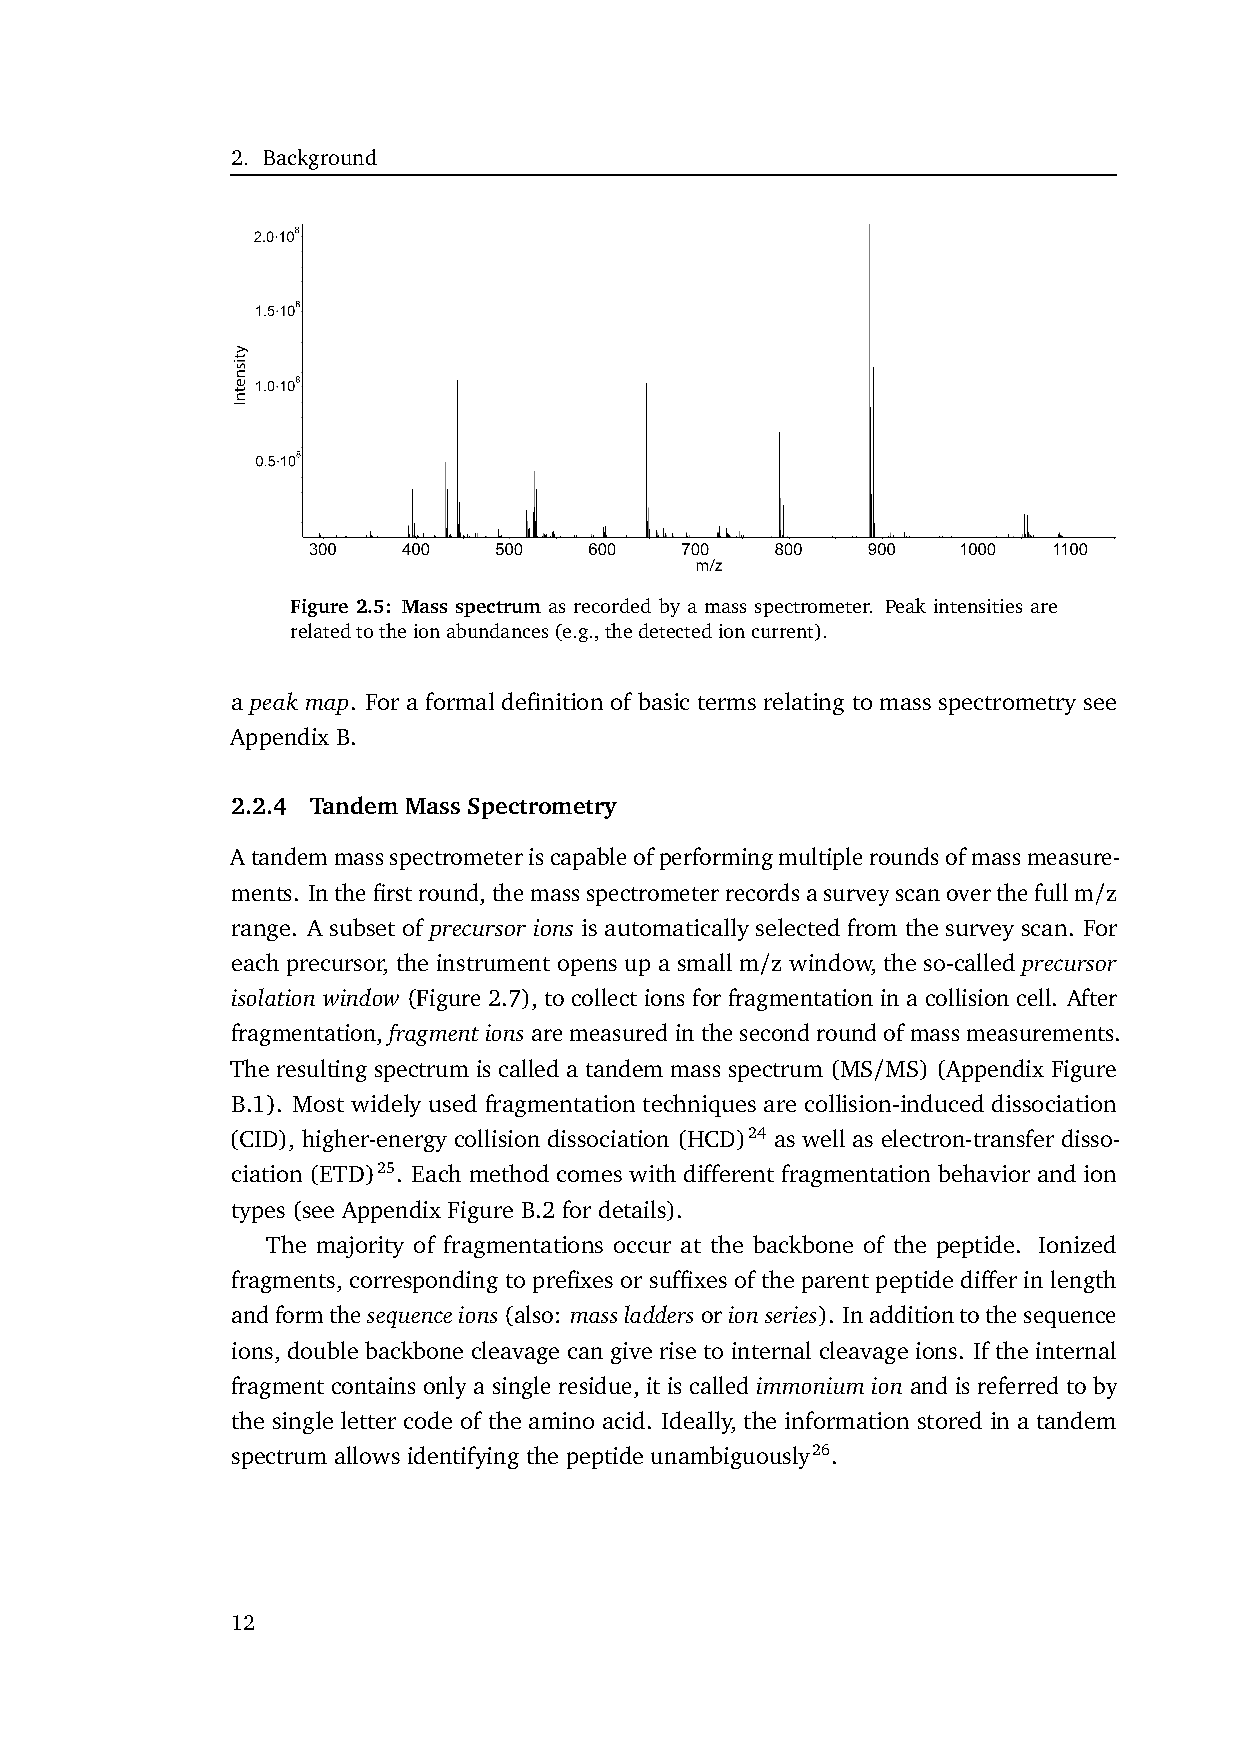
\includegraphics[width = \textwidth, trim=3.9cm 20cm 2.5cm 3cm,clip]{figures/Grafik_Timo.pdf}
		\label{fig:mass_spectrum}
		\caption[Example for a mass spectrum]{Example for a mass spectrum as recorded by a mass spectrometer. The ion intensity correlates with the amount of a molecule in the sample, $\frac{m}{z}$ is the mass-to-charge-ratio. From:~\citet{Sachsenberg2017}}
	\end{figure}
	}
	Because mass alone does not give enough information about a peptide to determine its sequence, tandem mass spectrometry is often used to gather more detailed evidence. In this procedure, particles of similar $\frac{m}{z}$ ratio are selected for fragmentation in a collision cell after the first round of mass measurement~\cite{Sachsenberg2017}. In there, the substance collides with a gas to be broken down into smaller molecules. For proteins, fragmentation happens predominantly in their backbone, producing all possible sub-sequences of the peptide. This produces a spectrum that is almost unique for its protein, which allows for peptide identification using bioinformatics tools~\cite{Angel2012}.\\
	Algorithms like Sequest~\cite{Eng1994} or X!~Tandem~\cite{Craig2004} compare the resulting spectra with theoretical spectra calculated from a list of possible peptides and compute a score based on their similarity. The peptides are generated by obtaining a list of proteins expected in the sample and calculating the peptides resulting from the, for example enzyme-based, degradation of the proteins. The best scoring peptide is then considered a peptide-spectrum-match (PSM). The scores produced by those algorithms often do not distinguish well enough between correct and incorrect matches~\cite{Kll2007}, but they enable FDR estimation using decoy databases and serve as a basis for score re-calibration with the Percolator~algorithm~\cite{Kll2007, Granholm2012}.\\
	Decoy databases are created from the target database, contain usually as  many peptides~\cite{Peng2003, Moore2002} in a reversed or shuffled order with respect to the amino acid sequence~\cite{Aggarwal2016}. They are presented to the scoring algorithm either separately~\cite{Granholm2012} or mixed with the target database~\cite{Peng2003}. It is assumed, that decoy and target peptides have similar features~\cite{Moore2002} and are not easily distinguishable by a scoring algorithm. When the actually fitting peptide for a given spectrum is not in the target database, and thus a wrong one will be chosen, the best scoring peptide will be a decoy approximately half of the time. This allows for an estimation of wrongly assigned targets, since the score distribution is assumed to be the same for decoys and false targets~\cite{Aggarwal2016}.\\
	In practice, one estimates the probability of a PSM being a false target by counting the number of decoy-PSMs with the same or a higher score. It is then assumed, there are as many false targets and thus a false discovery rate (FDR) can be estimated. This leads to the following formula\footnote{In this thesis, the following approximation is used:\\
		$FDR \approx \frac{\text{\# decoy PSMs}}{\text{\# all PSMs}} = \frac{\text{\# decoy PSMs}}{\text{\# decoy PSMs} + \text{\# target PSMs}}$\\
		It is faster to calculate and yields results differing by the FDR, so in the relevant range of FDRs of $0$ to $5\%$ up to $5\%$:\\
		$\frac{\frac{\text{\# decoys}}{\text{\# targets}}}{\frac{\text{\# decoys}}{\text{\# decoys} + \text{\# targets}}} = \frac{\text{\# decoys} + \text{\# targets}}{\text{\# targets}} = 1 + \frac{\text{\# decoys}}{\text{\# targets}} \approx 1 + FDR$}~\cite{Granholm2012}:
	\begin{equation}
	FDR = \frac{\text{\# false target PSMs}}{\text{\# all target PSMs}} \approx  \frac{\text{\# decoy PSMs}}{\text{\# all target PSMs}}
	\end{equation}
	The q-value as a measure for a single PSM rather than a metric for a set of PSMs is then derived from this as the minimum FDR of all PSMs with a lower or equal score~\cite{Granholm2012, Aggarwal2016}. It will be used for estimating the credibility for any one PSM.\\
	As \citet{Kll2007} say, separating correct from incorrect target PSMs with already mentioned algorithms works fine, but there is still room for improvement. This is because often not all information is used and considered jointly. Percolator~\cite{Kll2007, Granholm2012} tries to utilize as much information as possible by using scores from different algorithms, features of the peptide like its length, of the spectrum or the PSM itself. It joins them using a linear SVM and a semi-supervised approach with cross-validation to retain as many PSMs as possible. In every iteration, the top ranking, non-decoy PSMs up to a certain threshold of q-value are chosen as positive training examples, and the decoy PSMs are used as negative training set. The PSMs are then re-ranked using the SVM score, with the intend of getting a better separation of true and false PSMs. If that holds true, the positive training set of the next iteration better is of higher quality and the SVM can be trained even better. The algorithm usually converges within the first 10 iterations~\cite{Kll2007}. To avoid having to split the data into training and testing set and consequently losing possibly correct PSMs but also avoid overfitting, a nested cross-validation approach is being used~\cite{Granholm2012}.



\cleardoublepage

%% Material and Methods
%%%%%%%%%%%%%%%%%%%%%%%%%%%%%%%%%%%%%%%%%%%%%%%%%%%%%%%%%%%%%%%%%%%%
% Grundlagen
%%%%%%%%%%%%%%%%%%%%%%%%%%%%%%%%%%%%%%%%%%%%%%%%%%%%%%%%%%%%%%%%%%%%

\chapter{Material and Methods}
\label{matmet}
\label{lab:matmet:dataset}
To be able to test the following implementations, a dataset containing $93,219$ PSMs was used. Its spectra result from UV-light cross-linked extract from the nucleus of HeLa cells, and these were matched against the nucleus proteins. For each spectrum, up to 4 matching peptides are recorded. The dataset was generated with OpenNuXL~1.0.\\
Of the PSMs, $51,521$ are cross-linked and $41,698$ linear peptides, $50,627$ are target and $42,592$ are decoy peptides. Every PSM has $52$ features, $2$ columns specifying the spectrum and $2$ columns describing the peptide and the protein it originated from, as well as one column indicating to the experimenter whether one entry is a target or a decoy PSM. The features contain the NuXL-score, which was computed from the scores of different algorithms~(see \ref{lab:background:bioinfo_tools}), and was used as a reference.
\renewcommand{\baselinestretch}{0.9}
\begin{figure}
	\normalsize
	\centering
	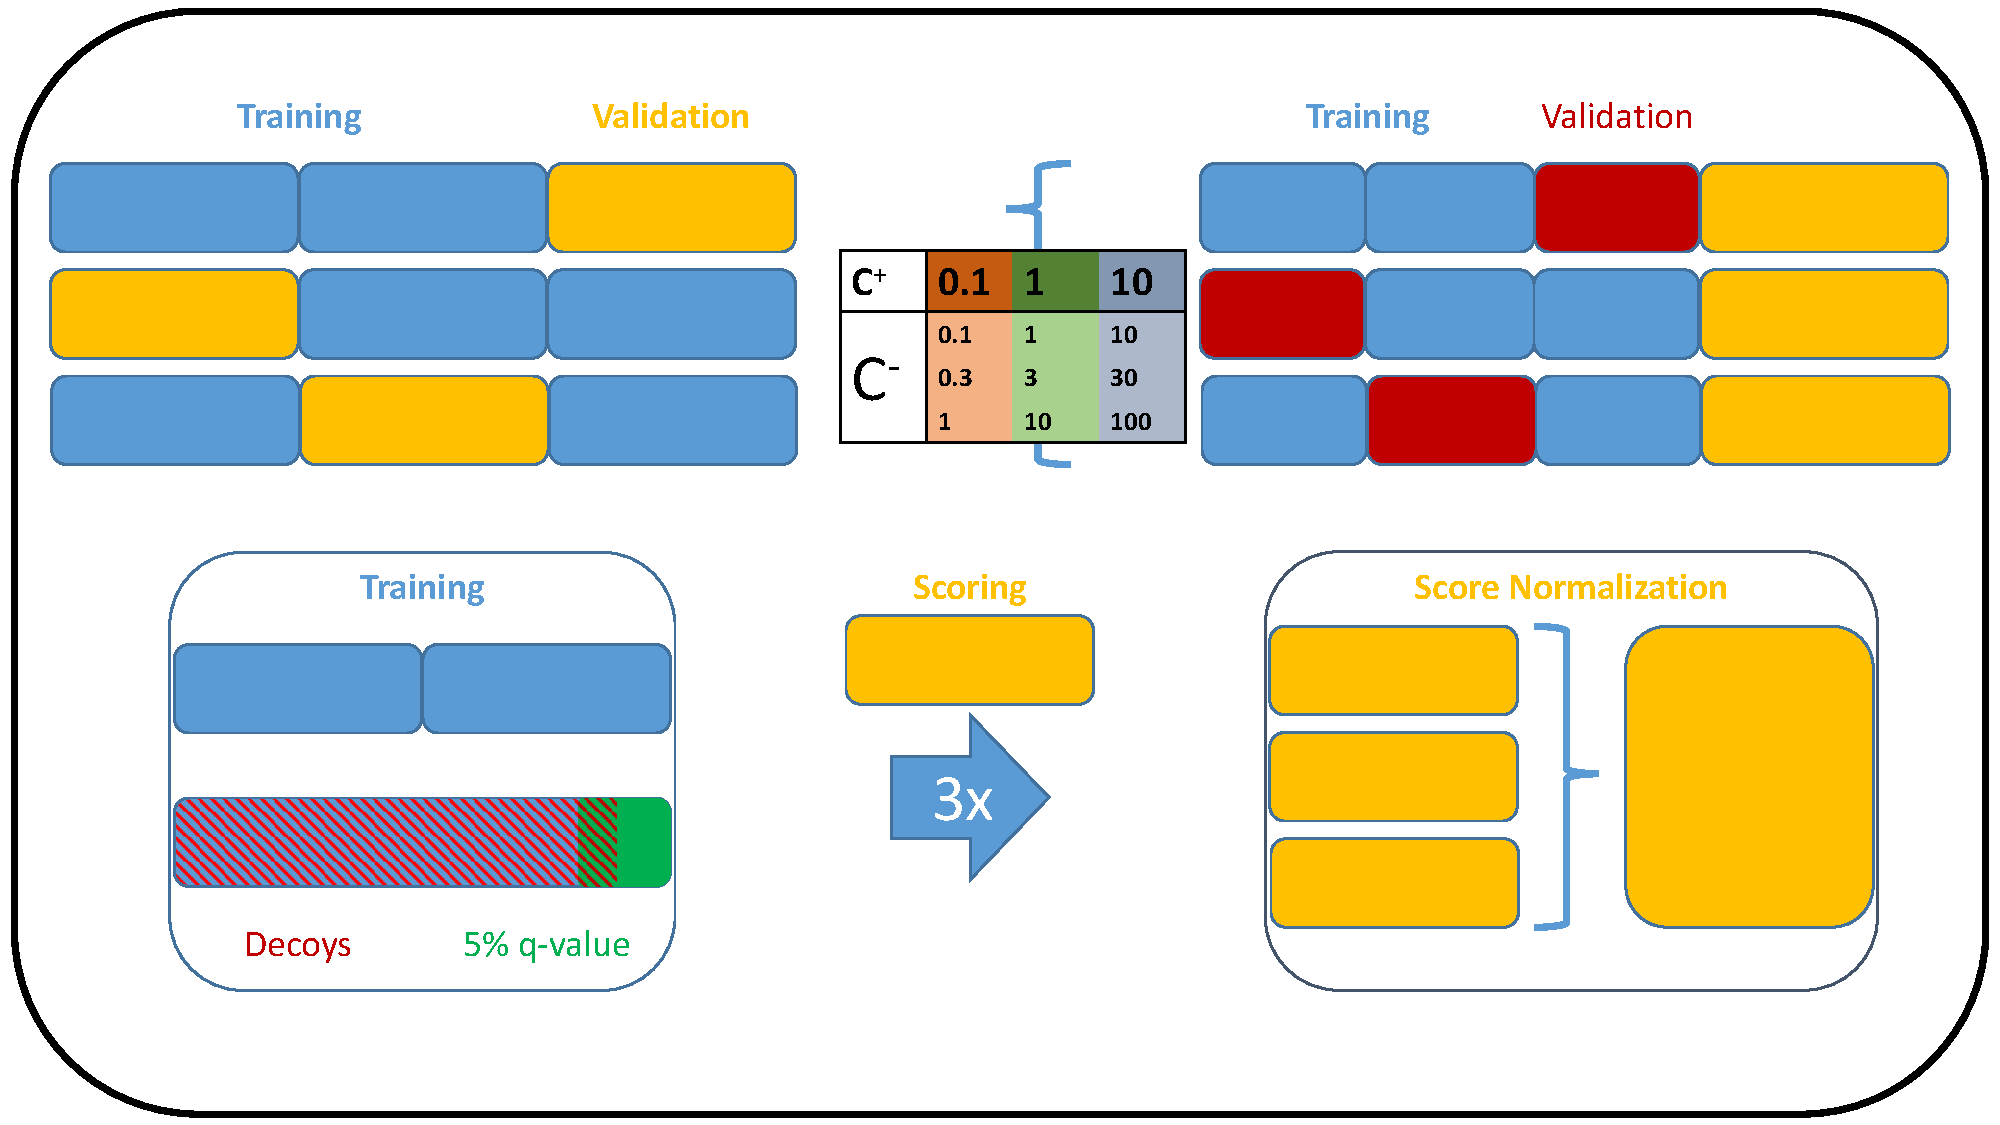
\includegraphics[width = \textwidth]{figures/Percolator_diagram.pdf}
	\caption[Procedure of Percolator]{Rough outline of the Percolator algorithm. First, the dataset is split in three parts, of which two are used for training and one for scoring. Then, another cross-validation is performed on the training part to determine the best parameter combination. Percolator searches the grid spanned by the options for the C parameter for positive examples $C^{+}$ ($0.1$, $1$ and $10$) and negative examples $C^{-}$ ($1$, $3$ or $10 \times C^{+}$). The parameter combination achieving best results on the training set is then used to train an SVM that scores the validation set. For training, all target PSMs with a q-value of $\leq 5\%$ are used as positive and all decoy PSMs are used as negative examples. Because in the end, the dataset will have been scored by three different SVMs, these scores have to be normalized. This is done by a linear transformation mapping the score representing a q-value of $1\%$ to $0$ and the median decoy score to $-1$. If \texttt{qScore} denotes the minimum score for which a q-value of $1\%$ is estimated and \texttt{dMedian} the median score a decoy achieves in the validation set, this sets score is transformed by the following equation: $\text{new Score} = \frac{\text{old score} - \text{\texttt{qScore}}}{\text{\texttt{qScore}} - \text{\texttt{dMedian}}}$.}
	\label{fig:percolator}
\end{figure}
\renewcommand{\baselinestretch}{1}\\

\section{Implementation of the Percolator algorithm}
The Percolator algorithm as presented in Figure~\ref{fig:percolator} was implemented in python. The pandas\footnote{https://pandas.pydata.org/} package was used for dataset handling, and for SVM calculations and inner cross-validation the classes LinearSVC\footnote{https://scikit-learn.org/stable/modules/generated/sklearn.svm.LinearSVC.html} and GridSearchCV\footnote{https://scikit-learn.org/stable/modules/generated/sklearn.model\_selection.GridSearchCV.html} from the python scikit-learn package were used. The outer cross-validation was implemented utilizing the numpy \texttt{array\_split}\footnote{https://numpy.org/doc/stable/reference/generated/numpy.array\_split.html} method. An early stopping criterion was implemented, terminating the algorithm if the area under the pseudo ROC curve does not improve over a certain number of iterations. This number is controlled by the parameter \texttt{termWorseIters} and has a default of 4.\\
\label{lab:matmet:normalization}As preprocessing, the provided file is read in as a pandas dataframe (converting strings to floating point or integer values if possible) and q-value and ranks are calculated as discussed in~\ref{lab:background:bioinfo_tools} and~\ref{lab:matmet:ranks} respectively. Also, the columns containing features are normalized. This means, their value is mapped linearly onto $[0,1]$ to avoid rounding errors in features of different orders of magnitude, caused by the representation of floating point numbers.\\
\label{lab:matmet:pseudoROC}For the calculation of pseudo ROC curves and the area under this curve, a function \texttt{pseudoROC} was implemented. It retrieves the entries of the given datasets q-value column, enumerates them and plots the enumeration against the q-values. This results in a pseudo ROC curve. Plotting was performed using the matplotlib.pyplot\footnote{https://matplotlib.org/api/pyplot\_api.html} package, and the area under the pseudo ROC curve was calculated by the scikit-learn auc\footnote{https://scikit-learn.org/stable/modules/generated/sklearn.metrics.auc.html} method.\\
To distinguish the original Percolator algorithm from the version implemented in python and altered here, the latter will be called Pycolator.

\section{Adapting Percolator to Cross-link Identification}
To be able to monitor the difference any experiment makes, especially with respect to the cross-linked or non-cross-linked PSMs, following features were implemented:\\
First, in addition to the q-value, which is calculated as described in~\ref{background}, the calculation of a class-specific q-value was implemented. This is done by splitting the dataset according to the class affiliation and calculating the q-value separately for both splits. This allows a more precise performance estimation when looking at only one of the classes.\\
\label{lab:matmet:rocs_after_every_iteration}
Second, an ROC curve using the \texttt{pseudoROC} function~(\ref{lab:matmet:pseudoROC}) is plotted after every iteration of Pycolator: one for the whole dataset, one only for cross-linked, and one only for non-cross-linked PSMs. Accordingly, the respective class-specific q-value is used. Thus, three plots covering the corresponding class(es) and every iteration, as well as the area under the curve are returned. This allows for fast visual detection of the impact a specific change to the algorithm has on certain classes, iterations or general sensitivity.
\subsection{Different Ranks}
\label{lab:matmet:ranks}
As experience shows, cross-linked peptides can be harder to detect than linear peptides. This means, the possibly correct cross-linked peptide will frequently not get the highest score of all the peptides. It thus can be beneficial to not only consider the highest scoring peptide, but also the highest scoring cross-linked peptide or also some lower-scoring peptides, and assign them ranks. Then, as following experiments show, Pycolator can correct the scores of some lower-ranking PSMs, possibly detecting more cross-linked PSMs. Meanwhile it is known to the experimenter, that only one of the peptides can be the correct match to a spectrum, and thus any PSM with a lower rank than 1 should be excluded at the end.\\
To tackle both constraints, Pycolator first trains the SVM with every PSM available and re-calculates the ranks based upon the newly assigned score after every iteration, possibly correcting the ranks of some PSMs. When the used metric, normally the area under the pseudo ROC curve, does not improve beyond a certain threshold per iteration, every PSM with rank $2+$ is dropped. The threshold is controlled by the parameter \texttt{cutOffImprove} with a default of $0.01$ corresponding to a $1\%$ increase of the used metric per iteration. Since also some of the best scoring PSMs will be dropped (even though they were not assigned rank 1), the algorithm then runs further until the maximum iterations are reached or the score does not improve further, in order to properly integrate and score the new PSMs considered confident. This procedure is depicted in Figure~\ref{fig:optimalRanking_outline}\\
The performance of this feature was tested against dropping the lower ranking PSMs once at the very end of the algorithm and once at the very beginning. Pycolator was run on the given dataset~(\ref{lab:matmet:dataset}) and pseudo ROCs were plotted as described in~\ref{lab:matmet:rocs_after_every_iteration}.
\renewcommand{\baselinestretch}{0.9}
\begin{figure}
	\normalsize
	\centering
	\includegraphics[width = \textwidth, page=2]{figures/Pycolator_diagram.pdf}
	\caption[Procedure of dealing with ranked PSMs]{}
	\label{fig:optimalRanking_outline}
\end{figure}
\renewcommand{\baselinestretch}{1}\\
\subsection{Characteristics of Cross-linked PSMs}
Apart from being hard to detect, cross-linked peptides also have other characteristics, some of which pose problems to the computational detection of correct PSMs. As discussed in~\ref{lab:matmet:splitting}~"Splitting the dataset", the features of cross-linked and linear peptides are so dissimilar, splitting the dataset and training a linear SVM separately on cross-linked and non-cross-linked~PSMs yields significantly better results than training one linear SVM. To reduce the impact of this heterogeneity, the following experiments were conducted:
\subsubsection{Proportions of Different Classes}
\label{lab:matmet:proportions}
As discussed in~\ref{lab:background:percolator}, Percolator employs a nested cross-validation approach, splitting the dataset, training on all parts than one and testing/scoring on the remaining part. If the splitting was uneven by chance, the SVM would be trained badly and the scoring inaccurate. Having different classes with significant differences in the dataset, like in our case cross-linked and linear PSMs or targets and decoys, increases this problem. For example, if there was a testing split with many cross-linked PSMs, the SVM had to be trained on the remaining data with few cross-linked PSMs, resulting in probably poor scoring of the many cross-linked PSMs in the test set. In the average case, this should not be a problem, but it can occasionally produce worse or better results, which would follow from overfitting.\\
To solve this problem, a mechanism of maintaining the proportion of the classes in the whole dataset for every inner and outer split was implemented. It can be toggled for targets and decoys or cross-linked and non-cross-linked PSMs as well as for inner and outer split independently. The impact was measured by running the algorithm $10$ times, plotting and recording the results of the best, worst and median run w.r.t. to the area under the pseudo ROC curve. Because this took approximately 90 minutes, the test was performed in a Google Colaboratory notebook\footnote{The Google Colaboratory notebook used:\\ \url{https://colab.research.google.com/drive/1VqZAmdta57YhgobA0WkQMqe_U9YIUnDl?usp=sharing}}.
%\begin{figure}
%	\label{fig:fluctuation_of_percolator}
%	\centering
%	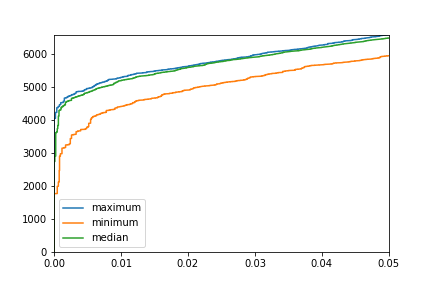
\includegraphics[width = 0.7\textwidth]{figures/percolator_MaxMinMedian_ClassesOption=.png}
%	\caption[Fluctuation of an earlier version of Percolator]{Pseudo ROC curve of an earlier version of the Percolator algorithm. It was run $10$ times and the best, worst and median run were plotted. Although the best run is close to the median one, the worst run is off by almost $1000$ PSMs. }
%\end{figure}
\subsubsection{Imputation}
\label{lab:matmet:imputation}
Cross-linked PSMs naturally have features linear PSMs do not have, which can however be used for training the SVM. An example would be the nucleotide it was linked to, or the partial loss score, which is the X!~Tandem~\cite{Craig2004} hyper score for the cross-linked peaks. In the given dataset~(\ref{lab:matmet:dataset}), $16$ out of $61$ features were only given for cross-linked PSMs. Optimally, these should not influence the score a non-cross-linked PSM gets. However, $0$ was filled in for the missing values and because that is a valid value for the linear SVM, it biases the decision made. For example, if a high value in a feature leads the SVM to a decision against the PSM, $0$ as the lowest value possible after feature normalization~(\ref{lab:matmet:normalization}) will tell the SVM to give the PSM a higher score. The procedure of replacing missing values with numbers minimizing the bias is called imputation. The scikit-learn package provides methods for the implementation in python\footnote{https://scikit-learn.org/stable/modules/impute.html}, and one of these, the \texttt{IterativeImputer}~function, was tested.
\subsubsection{Splitting the Dataset}
\label{lab:matmet:splitting}
Because the SVM is linear, one feature can not alter the influence another feature has on the decision. Thus, splitting the dataset into cross-linked and non-cross-linked PSMs should allow the SVM to fit more precisely onto the characteristics of each. This was tested by running Pycolator on each split and then concatenate the datasets, recalculating the q-values from the Pycolator scores. It was also tested splitting the dataset by the nucleotide the peptide was cross-linked onto, and non-cross-linked PSMs as a fifth class.
\subsection{Small datasets}
\label{lab:matmet:small_datasets}
The portion of cross-linked PSMs in a dataset is often very small. To evaluate when splitting as proposed in~\ref{lab:matmet:splitting}~"Splitting the Dataset" is possible and obtain general insight into the scalability of Pycolator, two experiments were conducted to conclude how small a dataset may be, so that the Percolator algorithm still works. In each case, Pycolator was applied to a dataset sampled from the given one~(\ref{lab:matmet:dataset}). The area under the pseudo ROC curve and the number of PSMs identified at $1\%$ q-value were recorded and used as metrics. The results achieved by Pycolator were compared to the effect the splitting had on the q-value estimation utilizing the given, precomputed NuXL score.\\
First, the smaller dataset was sampled using every $2^i$-th PSM from the whole dataset with $i\in\mathbb{N} \land i\in[0,13]$. Second, the smaller dataset was sampled randomly using a uniform distribution from all PSMs with a q-value of~$<10\%$. The portions sampled were $\frac{1}{2^i} : i\in\mathbb{N} \land i\in[0,12]$. Additionally to the metrics mentioned above, also the expected number of identifications at $1\%$~q-value for each split were calculated and recorded. This was done by counting the number of such PSMs before re-estimating the q-value or letting Pycolator run, thus being the number of identifications by the NuXL score if the q-value is estimated based on the whole dataset.
%For the NuXL score as reference and the Pycolator score respectively one plot showing the portion of PSMs with a q-value of $1\%$ and one plot showing the ratio of found to number of expected PSMs with $1\%$ q-value as a function of the dataset size were generated. In the end, the ratio of AUCs and identifications at $1\%$ q-value generated by the NuXL vs Pycolator score were plotted as a function of the dataset size. 
To compensate for the randomness in this experiment, Monte-Carlo-Sampling with 10 iterations was performed and the results are presented with boxplots. Because Pycolator re-ranks PSMs and then drops the ones with a lower rank than $1$, the dataset sizes are not equal in every of the $10$ iterations, and differ from the sizes when Pycolator is not run. Only one resulting size of each split is drawn as x-labels, and to still be able to compare the results after Pycolator is run and before, the metrics are used as proportion of dataset size.\\
Because numerical problems occur when calculating the area under a pseudo ROC curve of a very small dataset (since the curve can consist of only one point), another metric was introduced: the number of identified PSMs at a q-value threshold of $1\%$. Per default, Pycolator decides automatically after its first iteration if this metric is required based on the dataset, and adjusts its log, plots per iteration and functions like the early stopping criterion accordingly.\\\\
%(- Performance auf anderem Datensatz\\
%- Vergleich mit Entrapment FDR)
\cleardoublepage

%% Results
\chapter{Results}
\label{results}


\section{Implementation of the percolator algorithm}
- Reimplementierung funktioniert wie Original\\
- feature normalization war wichtiger boost\\
- ROC nach jeder Iteration zeigen

\section{Adapting Percolator to Cross-link Identification}
\subsection{Different Ranks}
- Ergebnisse von OptimalRanking\\
Before the implementation of the new procedure, ...\\
After the implementation [difference]
\renewcommand{\baselinestretch}{0.9}
\begin{figure}
	\normalsize
	\centering
	\begin{subfigure}{0.45\textwidth}
	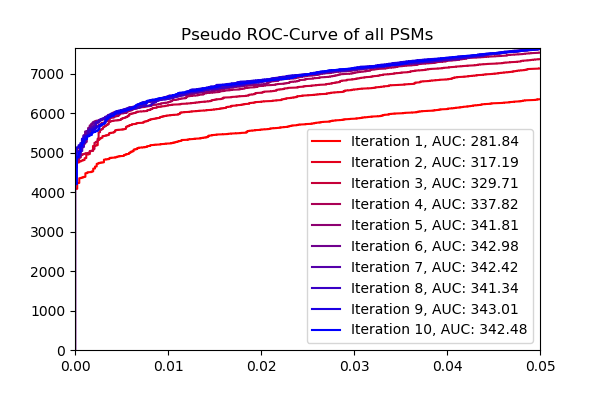
\includegraphics[width = \textwidth]{figures/allRanks.png}
	\caption[Result of dropping lower ranks at the end]{}
	\label{fig:all_ranks}
	\end{subfigure}
	\hfill
	\begin{subfigure}{0.45\textwidth}
	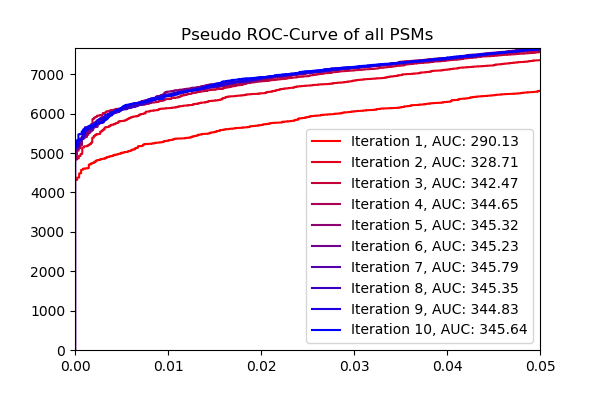
\includegraphics[width = \textwidth]{figures/onlyFirstRank.png}
	\caption[Result of dropping lower ranks at the start]{}
	\label{fig:only_rank_one}
	\end{subfigure}
\end{figure}
\renewcommand{\baselinestretch}{1}

\subsection{Characteristics of Cross-linked PSMs}
\subsubsection{Proportions of Different Classes}
\label{lab:results:proportions}
- Verhältnis Targets:Decoys und XL:non-XL verringt die Streuung: MinMaxMedian Auswertungen\\
\subsubsection{Imputation}
\label{lab:results:imputation}
- Bei Imputation kam nichts heraus\\
\subsubsection{Splitting the Dataset}
\label{lab:results:splitting}
- Großer Unterschied wenn man den (großen) Datensatz nach XL/nXL oder sogar cross-linking target aufteilt\\

\subsection{Small datasets}
- Sinnvolle Plots zu Ratio Testing\\
- Neue Metrik erlaubt es der Implementierung, auch auf kleineren Datensätzen zu funktionieren
\cleardoublepage

%% Discussion and Outlook
%%%%%%%%%%%%%%%%%%%%%%%%%%%%%%%%%%%%%%%%%%%%%%%%%%%%%%%%%%%%%%%%%%%%
% Diskussion und Ausblick
%%%%%%%%%%%%%%%%%%%%%%%%%%%%%%%%%%%%%%%%%%%%%%%%%%%%%%%%%%%%%%%%%%%%

\chapter{Discussion and Outlook}
\label{discussion}

- Methoden hinterfragen oder begründen, Ergebnisse interpretieren, Anwendbarkeit diskutieren, z.B.:\\
- Warum habe ich mich mit Rängen beschäftigt? (Bei XL-Datensätzen oft sinnvoll um erst percolator entscheiden zu lassen was auf Rang 1 steht (?)) -> Timo: "XL sind schwer. Richtiger XL oft auf Rang 2+, d.h. man muss alle Daten nutzen (= Percolator benutzen) um die maximale Anzahl an XLs zu identifizieren\\
- Falsche Formel für q-value\\
- C Parameter für jeden split neu optimieren führt zu overfitting? $\rightarrow$ Original-Algorithmus macht es auch so\\
- Wie sinnvoll ist die neue Metrik (idents bei 1\%)?\\
% NUR FALLS MAN DAS IN DEN ERGEBNISSEN SIEHT: onlyUseRankOne war lange bestes Ergebnis $\Rightarrow$ Schlechtere Ränge verwirren percolator? $\rightarrow$ Nein: Standard in pseudoROC-Funktion hat von sich aus Ränge gefiltert, was ich nicht beachtet habe (Macht so ein Punkt Sinn? War ja eigentlich nur ein Fehler meinerseits, den man aber evtl. in den Ergebnissen sieht...)\\
- ScanNr Versuche: Gleiche Spektren (identifiziert anhand der ScanNr.) auf verschiedene splits verteilen verändert nichts, d.h. vermutlich sind die niedrigeren Ränge dann so schlecht, dass es nichts bringt die schonmal gesehen zu haben.\\
- Peptide Versuche: Schlechtere Ergebnisse, aber vllt ehrlicher?\\
%Die Generalisierung von manchen Peptiden auf alle Pepide fällt der SVM schwer, weil der score sinkt wenn man die Peptide im test set nicht auch im train set zeigt.\\
%auf was soll man aber noch generalisieren, die svm wird gelöscht sobald der split fertig ist. Ist es hier unehrlich oder besseres training, wenn man der svm gute Beispiele zeigt?\\		
%Idee: Vielleicht sind es nur wenige, bestimmte Peptide (oder Proteine), die besondere Eigenschaften haben und somit schlecht vorhergesagt werden können?\\
%Oder: Peptide von decoys und peptide von targets sind disjunkt. Vielleicht haben gleiche Peptide gleiche Eigenschaften in manchen der scores, und die SVM kriegt diese Eigenschaften über die false train mit? Und kann somit zwischen decoy und target direkt unterscheiden?\\
%$\rightarrow$ weitere Experimente? Zu beachten: nXL werden hier immer schlechter!\\
- Mögliche weiterführende Experimente: mächtigere Klassifikatoren + monotonic constraints (wie von Timo ausprobiert), Ada-Boosting, feature selection

\cleardoublepage


%%%%%%%%%%%%%%%%%%%%%%%%%%%%%%%%%%%%%%%%%%%%%%%%%%%%%%%%%%%%%%%%%%%%%%%%%%%%%
%%% Bibliographie
%%%%%%%%%%%%%%%%%%%%%%%%%%%%%%%%%%%%%%%%%%%%%%%%%%%%%%%%%%%%%%%%%%%%%%%%%%%%%

\addcontentsline{toc}{chapter}{Bibliography}

\bibliographystyle{plainnat}
\bibliography{bibliography}

\cleardoublepage

%%%%%%%%%%%%%%%%%%%%%%%%%%%%%%%%%%%%%%%%%%%%%%%%%%%%%%%%%%%%%%%%%%%%%%%%%%%%%
%%% Erklaerung
%%%%%%%%%%%%%%%%%%%%%%%%%%%%%%%%%%%%%%%%%%%%%%%%%%%%%%%%%%%%%%%%%%%%%%%%%%%%%
\thispagestyle{empty}
\section*{Selbst\"andigkeitserkl\"arung}

Hiermit versichere ich, dass ich die vorliegende Bachelorarbeit 
selbst\"andig und nur mit den angegebenen Hilfsmitteln angefertigt habe und dass alle Stellen, die dem Wortlaut oder dem 
Sinne nach anderen Werken entnommen sind, durch Angaben von Quellen als 
Entlehnung kenntlich gemacht worden sind. 
Diese Bachelorarbeit wurde in gleicher oder \"ahnlicher Form in keinem anderen 
Studiengang als Pr\"ufungsleistung vorgelegt. 

\vskip 3cm

Ort, Datum	\hfill Unterschrift \hfill 


%%% Ende
%%%%%%%%%%%%%%%%%%%%%%%%%%%%%%%%%%%%%%%%%%%%%%%%%%%%%%%%%%%%%%%%%%%%%%%%%%%%%

\end{document}

